%; whizzy chapter
% -initex iniptex -latex platex -format platex -bibtex jbibtex -fmt fmt
% 以上 whizzytex を使用する場合の設定。

%     Tokyo Debian Meeting resources
%     Copyright (C) 2006 Junichi Uekawa

%     This program is free software; you can redistribute it and/or modify
%     it under the terms of the GNU General Public License as published by
%     the Free Software Foundation; either version 2 of the License, or
%     (at your option) any later version.

%     This program is distributed in the hope that it will be useful,
%     but WITHOUT ANY WARRANTY; without even the implied warranty of
%     MERCHANTABILITY or FITNESS FOR A PARTICULAR PURPOSE.  See the
%     GNU General Public License for more details.

%     You should have received a copy of the GNU General Public License
%     along with this program; if not, write to the Free Software
%     Foundation, Inc., 51 Franklin St, Fifth Floor, Boston, MA  02110-1301 USA


%   Pdf作成手順
% dvipdfmx debianmeetingresume200510.dvi

%%ここからヘッダ開始。

\documentclass[mingoth,a4paper]{jsarticle}
\usepackage[dvipdfmx]{graphicx}
\usepackage{fancybox}
\usepackage{longtable}
\usepackage{ascmac}	% 囲み (screen,itembox)
\usepackage{fancyvrb}   % 囲み Verbatim のために必要
\usepackage[dvipdfmx]{hyperref}
\usepackage{url}

%http://www.naney.org/diki/dk/hyperref.html
%日本語EUC系環境の時
\AtBeginDvi{\special{pdf:tounicode EUC-UCS2}}
%シフトJIS系環境の時
%\AtBeginDvi{\special{pdf:tounicode 90ms-RKSJ-UCS2}}

%% spacing の設定をする。外枠を減らす。
\setlength\headheight{0mm}
\setlength\topmargin{-20mm}
\setlength\headsep{0mm}
\setlength\topskip{3mm}
\setlength\maxdepth{4pt}
\setlength\columnsep{6mm}
\setlength\textheight{252mm}
\setlength\topmargin{-5mm}
\setlength\textwidth{170mm}
\setlength\oddsidemargin{-5mm}
\setlength\evensidemargin{-5mm}

% commandline環境を定義。画面入出力についてはcommandline環境
% で表記する
\newenvironment{commandline}%
{\VerbatimEnvironment
  \begin{Sbox}\begin{minipage}{15cm}\begin{fontsize}{7.3}{7.3} \begin{BVerbatim}}%
{\end{BVerbatim}\end{fontsize}\end{minipage}\end{Sbox}
  \setlength{\fboxsep}{8pt}\fbox{\TheSbox}}

% 三択問題用
\newcounter{santakucounter}
\newcommand{\santaku}[4]{%
\addtocounter{santakucounter}{1}

\nopagebreak 問題\arabic{santakucounter}. 
#1\\
\nopagebreak□ A #2\\
\nopagebreak□ B #3\\
\nopagebreak□ C #4
\pagebreak[1]
\hspace{1cm}
\\

}

\newcommand{\emptyspace}{(\underline{\hspace{1cm}})}



\newcommand{\subsubsubsection}[1]{%
\vspace{1zw}{\bf #1}\\}


% sectionをセンタリングする
\makeatletter
  \renewcommand{\section}{\@startsection{section}{1}{\z@}%
    {\Cvs \@plus.5\Cdp \@minus.2\Cdp}% 前アキ
    {.5\Cvs \@plus.3\Cdp}% 後アキ
    {\normalfont\Large\headfont\raggedright\centering}} % style
\makeatother

% section の代わりの環境
\newcommand{\dancersection}[2]{%
\newpage
東京エリアDebian勉強会 2005
\hrule
\vspace{0.5mm}
\hrule
\hfill{}
\includegraphics[width=3cm]{image200502/openlogo-nd.eps}\\
\vspace{-4cm}
\begin{center}
  \section{#1}
\end{center}
\hfill{}#2\hspace{3cm}\space\\
\hrule
\hrule
\vspace{1cm}
}

% BTSの番号を見るためのコマンド
\newcommand{\debianbug}[1]{Bug\##1\footnote{\url{http://bugs.debian.org/#1}}}

%%

\begin{document}


\begin{titlepage}


% 毎月変更する部分, 本文の末尾も修正することをわすれずに
\title{
 第9回 東京エリア Debian 勉強会\\事前資料}
\date{2005年10月15日}
\author{Debian勉強会会場係 上川 純一\thanks{Debian Project Official Developer}} 
\maketitle
\thispagestyle{empty}

\end{titlepage}

\newpage
\tableofcontents

\dancersection{Introduction To Debian 勉強会}{上川 純一}

今月のDebian勉強会へようこそ。
これからDebianのあやしい世界に入るという方も、すでにどっぷりとつかってい
るという方も、月に一回Debianについて語りませんか?

目的として下記の二つを考えています。

\begin{itemize}
 \item メールではよみとれない、もしくはよみとってられないような情報を情
       報共有する場をつくる
 \item まとまっていないDebianを利用する際の情報をまとめて、ある程度の塊と
       して出してみる
\end{itemize}

また、東京にはLinuxの勉強会はたくさんありますので、Debianに限定した勉強
会にします。Linuxの基本的な利用方法などが知りたい方は、他でがんばってくださ
い。
Debianの勉強会ということで究極的には参加者全員がDebian Packageを
がりがりと作りながらスーパーハッカーになれるような姿を妄想しています。

Debianをこれからどうするという能動的な展開への土台としての空間を提供し、
情報の共有をしたい、というのが目的です。
次回は違うこと言ってるかもしれませんが、御容赦を。

\subsection{講師紹介}

\begin{itemize}
 \item{樽石さん} apt-listbugsを開発した人です。
 \item{上川 純一} 宴会の幹事です。
\end{itemize}

\subsection{事前課題紹介}

% workflow: tokyodebian-2005@lists.alioth.debian.orgを確認
% debianmeeting-2005@mlist11.netfort.gr.jpを確認

今回の事前課題は
「Debianのバグシステムに物申す」
というタイトルで200-800文字程度の文章を書いてください。
というものでした。
その課題に対して下記の内容を提出いただきました。

\subsubsection{澤田さん}

特に物申すことがないので勉強会に先駆けてapt-listbugsのコードを読んでみま
した。ふ〜む、osdn.debian.or.jpに置いてある
\verb!index.db-#{severity}.gz!を拾っ
てきてcriticalやgraveなバグを取得、さらに
\verb!#{bug_number}.status!を拾ってバ
グ情報を取得しているのか・・・、ということはapt-listbugsのリクエストはす
べてosdn.debian.or.jpに行っているということになり結構な負荷がかかってい
るのではないかと思う。問題ない程度なのか、問題があるけど何らかの回避方法
を使っているのかが聞ければいいな〜と思う。index.dbとstatusをミラーに置く
ようにしてapt-listbugsはsources.listに書かれているミラーからindex.dbと
statusを取得するようにするなんてどうなんだろうか。

\subsubsection{えとーさん}

広い意味での Debian のバグシステムの話になるが、
セキュリティの報告などがCVEに重点を置かれているが、
CVEはUS-CERT
\footnote{
US-CERTについて
\url{http://www.us-cert.gov/aboutus.html}

The United States Computer Emergency Readiness Team (US-CERT) 
is a partnership between the Department of Homeland Security 
and the public and private sectors. Established in 2003 to protect 
the nation's Internet infrastructure, US-CERT coordinates defense against 
and responses to cyber attacks across the nation.
}
はあくまでアメリカの
国内向けのセキュリティ情報を扱う組織が行なっているので
例えばJPCERT/CCとの連携などには積極的ではない。
JPCERTが現状だめだ、というだけでなく重点がUS-CERT発行の
ものなのでどうしても、差が出てしまいこまったことに
なるのはどうにかならないのかなぁ。
バグシステムについてはドキュンバグのフィルタリングは
当該メンテナがやらなければいけないが、他の人からも
評価というか注目度の上げ下げを付けられるようにすると
よいのでわないだろうか。

\subsubsection{中島さん}

 バグ報告できるのか!けれど英語で報告しなくてはならないのは、けっこう大変だか
ら報告はしない。というよりできない。めんどうだから。それよりも、まずバグがよ
くわからない。「これはバグなのか?」というのがあるわけだし、自分自身が間違っ
てるかもしれないわけで、なのでバグがあったら自動的に報告するというのがいいと
思う。バグだ。と思う前に勝手にコンピュータがバグ報告を送信するのだ。これで使
えば使うほどバグがなくなるはずだ。これがいい。

\subsubsection{小林さん}

個人的には、Debianのバグ追跡システム (BTS) にそんなに不満はありません。
白い背景に黒い文字という、何の工夫もない見かけが少し悲しいと思っていましたが、
最近ではスタイルシートが適用されて少しよくなったようにも思います。

初めてバグ報告したときに嬉しかったのは、reportbugパッケージの存在でした。
好みの問題もあるでしょうが、
MUA を開いてメールを書かなくてもコマンドラインからバグ報告ができるのは、
非常に嬉しいことです。

ただ、つい数日前に久し振りにバグ報告をして初めて気付いたのですが、
sargeのreportbugコマンドでバグを送信しようとしたときに、
「12 bug reports found:」のようなものは出ても、
その下に既存のバグ報告のリストが出てこなくそのままバグ報告内容の編集に移ります。
woodyのはエラー終了します。
2005年7月の機能追加か何かのせいでしょうか?
リリースされたばかりの安定版のreportbugの機能の一部に明確な問題が出るのは残念です。

reportbugは、あくまでBTSのウェブインタフェースをパースし、
コマンドラインからのバグ報告を可能にしてくれるツールだと思います。
しかしそれだと、
今回のようにウェブインタフェースが変化してしまった場合に使えなくて困るので、
もう少しBTSと一体化した、
ウェブインタフェースに依らない (異なるインタフェースを使った) reportbugの仕様、
またはreportbugによるパース結果が変わらないようなウェブインタフェースの仕様が好ましいと感じました。

まぁ、バグ報告するなら不安定版を使えということなのかもしれませんが……。

\subsubsection{上川}

最近BTSの機能が改良して、いろいろと新しいことができるようになった。
見ためもかわって、いままでとどこおっていた開発が再開したのはよいことだと
思う。
ただ、従来の出力を解析していたツールがうまくうごかない。
自分のコードで動かなくなったのは、たとえばemacsでdebian/changelogを編集する
モードがあるのだが、そこでBTSからバグのタイトルと送信者の名前をとってき
てバグをcloseするためのchangelogエントリを書くというものがある。
それが最近どうも動いていないらしい。
ウェブページを正規表現で解析していたような記憶がうっすらとあるので修正し
たら一瞬で直るんだろうなぁ、とおもいつつもまだ修正するにいたっておりませ
ん。


%%% trivia quiz
\dancersection{Debian Weekly News trivia quiz}{上川 純一}

ところで、Debian Weekly News (DWN)は読んでいますか?
Debian 界隈でおきていることについて書いているDebian Weekly News.
毎回読んでいるといろいろと分かって来ますが、一人で読んでいても、解説が少
ないので、
意味がわからないところもあるかも知れません。みんなでDWNを読んでみましょう。

漫然と読むだけではおもしろくないので、DWNの記事から出題した以下の質問にこたえてみてください。
後で内容は解説します。

\subsection{2005年37号}
2005年9月13日です。
%http://www.debian.org/News/weekly/2005/37/
 \santaku{バグトラッキングシステムの見栄えで最近かわったのは何か}
 {CSSを利用するようになった}{DHTMLになった}{XHTMLになった}
 \santaku{Debian UKで問題になったのは何か}{メンバーが活動的でないこと}
 {UKの経済状況がよろしくないこと}{商用利用をしようとした場
 合のDebianという名前の商標の利用の許可をする基準が不明確だったこと}
 \santaku{ソフトウェアを計測する、という論文で発表されたのは何か}{Debian
 sarge には2億3000万行のソースコードが含まれている}{Debian sargeの品質を
 計測した}{Debian sargeの利用しやすさを計測した}
 \santaku{Joey Hess は testing に対して security 対応をすることを発表した。
 それに利用しているサーバはどれか}
 {secure-testing.debian.net}{security.debian.org}{security.debuan.org}
 \santaku{/usr/docをいまだにつかっているパッケージ数はどれくらいか}{100}{200}{500}%C
 \santaku{planet.debian.orgをメーリングリスト経由で配布しようという意見
 に対して出た反論は}{blogの内容は機密事項なので、メーリングリストで配布
 してほしくない}{メーリングリストとして配布するとサーバの負荷が高くなる}{blogの内容を永続的にメーリングリストのアーカイ
 ブとして保存されたくない}%C
 \santaku{/usr/share/doc/パッケージ名/examples/ にあるファイルに実行権限
 をつけることについてはどうするべきか}{サンプルは実行できるものは
 実行権限をつけるべき}{サンプルなんてかざりなので実行しなくてよい}
 {/usr/share以下について実行権限をつけるのはこのましくなく、実行ファイルはbinにおくべきだ。}
 \santaku{sponsors.debian.netが提供するサービスは何か}{金銭的寄付をつの
 るフィッシングサイト}{広告を配信し、広告収入をDebianプロジェクトの発展
 のために利用するサイト}{まだメンテナ
 になっていない人が管理しているパッケージについてスポンサーが必要な状況
 をトラッキングするシステム}
 \santaku{1.0beta3のようなベータ版のバージョン番号が1.0のような最終版の
 バージョン番号より低い、とdpkgが判定してしまう。この状況に関してメンテ
 ナはどう対応するべきか}
 {優先度の低い チルダ記号 \~{ }を利用して、 1.0\~{
 }beta3のような名前にする。
ただまだアーカイブシステムが対応していないので、今後の改善が必要。}{あき
 らめる}{ベータ版はパッケージ化しない}
 \santaku{ソースのみのパッケージのアップロードを可能にするという提案についての反論は
 何か}{バイナリが必要でなくなると、メンテナがテストをしなくなるのではな
 いだろうか、という懸念がある}{ソースのみだとパッケージインフラが破綻す
 る}{katieを改変するのが面倒}
 \santaku{BTSに任意のタグを追加できる機能が追加された、なんという機能か}
 {tagtag}{たぐるんです}{usertag}

\subsection{2005年38号}
2005年9月20日です。
%http://www.debian.org/News/weekly/2005/38
 \santaku{David Moreno Garzaがwnppにてcloseしたバグレポートの数は}{729の
 バグレポート}{100のバグレポート}{123のバグレポート}%A
 \santaku{International Conference on Open Source Systemsに投稿された論
 文の中で説明されていた結果は}{開発者は短期間でどんどん入れ替わる}{メン
 テナは実は幻想で、そんな人は存在しない}{長いあいだアクティブに活動し、パッケー
 ジの数も多くメンテナンスする} % c
 \santaku{Frank Lichtenheldが発表したのは、non-freeなドキュメントを削除
 する処理を開始するということだった。状況をトラッキングするために彼が利
 用したインフラは。}{BTSののusertags機能で
 debian-release@lists.debian.orgユーザのタグとして管理}{
 Wikiページ}{CVS管理のテキストファイル}% A
 \santaku{Software freedom day 05でDebian-womenが行って、
 結果として良かったので今後も継続することになったのは}{debian-women-new
 IRCチャンネルがよい結果をもたらしたので、今後はdebian-womenチャンネルに
 新人を歓迎する時間帯というのをもうける}{CDをたくさん焼いたら人気だった}
 {KatieやBTSなどをインストールしてユーザがいじれるように提供したら人気だったので、今後もやる}
 \santaku{init.dスクリプトは現在直列に実行されているが、今後
 、並列実行を実装する際に便利だろうと思われる
 LSB規格の仕様は}{なんとなく並列に実行しても壊れないようにする仕様}{
 気持の中だけでは並列な年頃}{initスクリプトの中で依存関係を記述できる仕様}
 \santaku{新しいバージョンのパッケージにて問題が解決した場合の、バグレポー
 トをクローズする方法でないのは何か}{changelogでバグ番号を記述し
 アップロードする}
 {バージョンヘッダを付けて、リクエストを -done アドレスに投げる}{btsclose
 コマンドを利用する} %c
 \santaku{Marc Brockschmidtが説明した、新規メンテナプロセスのFront Desk
 の変更とは}{
今後はより厳しい思想チェックを行う}{Debianに
 コントリビュートしていることが要件になり、何もしていない場合は、応募が
 取り消される}{年齢制限を設けます}
 \santaku{security.debian.orgで問題になったのは何か}{セキュリティーアッ
 プデートが遅い}{セキュリティーアップデートが嘘だった}{xfree86のセキュリ
 ティーアップデートがあまりにも高いネットワーク負荷を発生させてしまい、
 security.debian.orgがサーバとして機能しなくなってしまった。}
\subsection{2005年39号}
2005年9月27日です。
%http://www.debian.org/News/weekly/2005/39/
 \santaku{Ben HutchingがDebconfについて報告したのは}{もう終ってしまった
 事は忘れる}{忘れ物がありました}{DVDが入手可能に
 なった}
 \santaku{wiki.debian.orgへの移行で特に手動の労力が必要だったのはどこか}
 {すでにwiki.debian.netからwiki.debian.orgに移行してしまっているページが
 いくつかあったのでそれに対しての手動の対処}{kwikiからmoinmoinへデータ形
 式の変更}{ドメイン名の登録}%Aのつもり
 \santaku{initの時点では/がread-onlyでマウントされているが、その時点でデー
 タを保存するのにはどうしたらよいか。}{メモリファイルシステムを/runにマ
 ウントする}{/mnt以下にメモリファイルシステムをマウントする}{/をrwにマウ
 ントしなおす}
 \santaku{グラフィックライブラリ GLU の実装がDebian内で複数ある理由はな
 ぜか}
 {一部のコードが一部のハー
 ドウェアでしか動かないという状況が続いているから}
 {複数のパッケージをメンテナンスしているほうがかっこいいから}{メンテナの
 仲が悪いから}
 \santaku{Jeroen van Wolffelaarが提案したのは}{libc5を消す}{libc6を消す}
 {libc6.1を消す}%A
 \santaku{piupartsであきらかになる問題は}{purgeする際に、essentialでは
 ないパッケージに依存して、動作しないパッケージ}{インストールしても動かないパッ
 ケージ}{使ってみて使いにくいパッケージ}

\subsection{2005年40号}
2005年10月4日です。
%http://www.debian.org/News/weekly/2005/40/
 \santaku{DPLチームが今後検討する予定の問題について記録する媒体として選
 択したのは}{BTS}{IRC bot}{Wiki}
 \santaku{tetex 3.0はどういう状況になっているか}{今後も入る見通しがない}
 {うごかなくて困っている}{experimentalにアッ
 プロードされ、ライブラリのフリーズが完了したらunstableに入る}
 \santaku{Debian で配布するIA64アーキテクチャ向けのカーネルについて
 Dann FrazierがSMPじゃないカーネルのサポートを削除しようとした、何故か}
 {SMPじゃないといやだから}{時代はSMPです}{IA64で、SMPでないシステムがほ
 とんどなく、あまりテストされていない} 
% Chris LameterはSMPじゃないシス
% テムも仮想化環境用などで必要だろうと説明しているが、Debianがそれをすべ
% きかというと違うだろう。
 \santaku{Wolfgang Borgert によると
planet.debian.orgと、メーリングリストの利用方法の違いは}
{メーリングリストは古い技術なので今後はつかわなくなる}{blogはフレームされないで意見を述べることのできるメディアだが、議論す
るのはメーリングリストでして欲しい}{planet.debian.orgは安定していないの
で使わないで欲しい}
 \santaku{pbuttonsdは/dev/input/eventXXを利用しているが、どういう問題が
 あったか}{makedevが、最大32あるうちの4個しかデバイスファイルをつくっていなかっ
 たので、/devを静的に管理しているユーザは一部の機能を利用できていなかっ
 た。}
 {USB接続ではうまく認識できなかった}{電源ボタンがおされたらアプリケーショ
 ンがハングした。}

\subsection{2005年41号}
2005年10月11日です。
%http://www.debian.org/News/weekly/2005/41/
 \santaku{Debian securityで改善したのは}{バックエンドとフロントエンドの
 サーバを分割し、負荷に強い構成に変更した}{特定のユーザが負荷をかけられ
 ないようにスロットリングした}{セキュリティーパッチをリリースしないこと
 でサーバに負荷がかからないようにした}
 \santaku{Carlos Parra Camargoが報告したのは何か}{Wikiが悪意をもったユー
 ザにより書き換えられていたので前のバージョンを復活させた}{Wikiがおもし
 ろくないので改善しよう}{Wikiサーバがダウンしている}
 \santaku{mozilla 1.7.8に対してのセキュリティーアップデートはどういう形
 でリリースされたか}{1.7.10にバージョン1.7.8という名前をつけてリリースし
 た}{セキュリティーパッチをバックポートした}{セキュリティーホールのある
 機能を全てdisableにした}
 \santaku{複数のchrootで同じユーザ情報を利用するのに利用できる方法でない
 のは}{FUSEのshadow etc}{LDAP}{rm /etc/passwd}
 \santaku{ソースコードにローカルに適用したパッチをパッケージの
 アップグレード後も維持するためにはどうしたら一番楽か}
{自分でがんばる}{apt-srcを利用する}{パッチはあてない}
 \santaku{Jurij Smakovがリリースした文書は何か}{Debian Users Handlebook:
 Debianユーザをどうあつかえばよいのか、が書いてある}{Debian Developers
 Handlebook: Debian Developerをどう扱えば良いか、が書いてある。
}{Debian Linux Kernel
 Handbook: Debianでカーネルがどうビルドされているのか、が書いてある}
%http://kernel-handbook.alioth.debian.org/

\dancersection{最近のDebian関連のミーティング報告}{上川 純一}


\subsection{東京エリアDebian勉強会8回目報告}


前回開催した第8回目の勉強会の報告をします。

	  9月の第8回東京エリアdebian勉強会報告。
	  debconfの使い方や実装についてあつく議論がかわされました。
	  今回の参加人数は登録者が16名くらいで、実際に参加したのが14名くらいでした。

	  
	    DWN quizに関しては、今回も満点をとった方がちらほら。

	    鵜飼さんがdebconfについて説明しました。
	    開発をする際に、.configスクリプトを書くのに必要な事項などについて説明しました。
	    backupするための実装や、いろいろと細かい挙動の話しになると
	    けっこうすごい実装になっているのでみんなびっくりしていたのではないでしょうか。

	    やまねさんがdebian JPのウェブページをどうしたいのかということについて
	    説明しました。
	    ぜひコミットしていただきたいところです。
	    誰にむかってウェブをつくっていくのか、という議論もでてきましたが、
	    新しく開発者がどんどん参加できるような情報として、入り口としては必要な
	    ウェブページだろう、という意見がでていました。



\dancersection{apt-listbugs の生い立ちと実装}{樽石}
\label{sec:taruishi}
%% taruishiさんの記事はここから 
この文書は 2005 年 3 月に北京で開催された Asia Debian Mini-Conf
in Beijin で発表した資料の日本語訳です。

\subsection{はじめに}


Debian は 24 時間 365 日、多くの開発者によって日夜開発されている自由
なオペレーティングシステムです。わたしたちはこのような最新のスナップショットを
Debian のアップグレードフレームワークを使うことで簡単に共有することができ、
実際に、このフレームワークを利用して多くの人が最新の Debian スナップショット
を利用しています。

一方で、この最新スナップショットはときどき壊れることがあります。apt-listbugs
は、このような壊れたスナップショットからあなたのコンピュータを守るための仕組みです。

この短い文書では、apt-listbugs がどのようにコンピュータを守るのか、apt-listbugs
の生い立ち、実装について簡単に説明します。また apt-listbugs の抱えている
現在の問題点について紹介します。

\subsection{仕組み}

Debian には Debian バグ追跡システム(BTS) として知られる、Debian に関する
全ての問題が利用可能な中央管理型バグ追跡システムがあります。Debian のパッケージ
インストールフレームワークである APT は apt-get や aptitude 等を利用して
インストールやアップグレードを行う直前に BTS からこれらの問題を取得するために
apt-listbugs を呼び出します。apt-listbugs はどのパッケージがインストール
されるのか、またアップグレードされるのかを自動認識し、問題となるバグを見付けた場合は
その事をユーザに通知し、インストールを継続するか警告を出します。

このアプローチは、主にふたつの問題、ひとつはユーザの視点、もうひとつは開発者の視点
を解決します。

\subsubsection{ユーザの視点}

ユーザの視点は apt-listbugs のメインの目的です。APT フレームワークは
任意のパッケージを簡単にアップグレードすることができます。複雑な作業を
一切行わずに単に 'apt-get upgrade' と実行するだけです。これはすばらしい
機能ですが、一方でこのアプローチは壊れたパッケージさえも簡単にインストール
させてしまいます。多くの人が apt-get upgrade を利用しているため、
結果として世界中の Debian マシンが一瞬のうちに壊れてしまうことになります。

実際は、壊れたパッケージの情報は BTS に既に存在している可能性が非常に高いのですが
この情報が BTS にあるかどうかを毎回チェックしないといけないとしたら apt-get upgrade
による簡単なアップグレード作業は面倒な作業に一変してしまいます。これが
apt-listbugs が必要な理由です。apt-listbugs はそのような情報が BTS
にあるかどうかをあなたの代わりに毎回自動で行います。

\subsubsection{開発者の視点}

ふたつ目の目的は Debian 開発者のためのものです。基本的には、BTS は Debian
パッケージに関するあらゆる情報知るために利用できるすばらしいものです。もし
自分のパッケージにバグがあった場合、他のユーザが問題を BTS に報告してくれます。
開発者はいつでも、どこでも、この情報にアクセスすることができます。

しかし、仮に自分の環境ではたまたま発生しなかった致命的な問題が最新のパッケージ
に含まれてしまったとします。こうなると、多くのユーザは問題の深刻さを考慮して
急いでバグ報告をしようとします。それゆえ、たったひとつのバグに対して
非常にたくさんのバグ報告を受け取ることになってしまい、開発者はバグ報告の分類という
本質的でない作業に時間をとられ、本当に直したい致命的な問題の解決に長い時間
を要してしまうことになります。もし、ユーザがバグをレポートする前に似たような
レポートを閲覧することができれば、重複したレポートを送ることはなくなるでしょう。

\subsection{ヒストリ}

apt-listbugs はもともとユーザの視点をなんとかしたいという個人的な目的で
数年前に開発されました。ちょうどその時は、大学院を修了するために修士論文を
書かなければいけない時期でした。ところが、何を思ったか〆切の一週間前に
apt-get upgrade をしてしまったのです。結果、NFS が動かなくなり、この
問題を修正しなければいけなくなりました。このバグレポートをきちんとチェックして
いれば、このような問題にはあわなかったのですが、バグレポートを毎回チェック
するわけにはいきませんでした。なぜならいつインストールされるかわからない
致命的な問題のために毎回バグレポートをチェックするのは非常に大変な作業
だからです。

\subsubsection{CGI 問題}

apt-listbugs の最初のバージョンは Debian にすぐにアップロードすることは
できませんでした。その理由は apt-listbugs は BTS の CGI 出力を利用して
いたからです。CGI スクリプトはスクリプト言語で書かれていたため、もしこのパッケ
ージをアップロードすると、BTS サーバが非常に高負荷になってしまうことは容易に想像
できます。そこで、この apt-listbugs を利用したら同時にアクセスできるユーザ
数は何人程度なのか知るために CGI のパフォーマンスを測定することにしました。
結果は、1 パッケージのレポートを取得するのにかかる時間は約 1 秒でした。
BTS サーバは 2 台の CPU を備えていましたので、結局 1 秒に 2 つの
バグレポートしか取得できません。そのため、もし 10 個のパッケージをアップグレード
しようとしたら、レポートの取得に 5 秒かかってしまいます。これは非常に大きな
問題です。特に、BTS サーバは Debian のマスタサーバでしたから、もし Debian
ユーザ全員がそのサーバからバグレポートを取得したら、これはほとんど DoS アタック
のような状態に陥ってしまいます。

\subsubsection{強制キャッシュ}

最初に考えた解決法は CGI 出力のキャッシュを行うプロクシサーバを利用することでした。
プロキシサーバが http の No-Cache 属性を無視すれば、静的なデータを利用することが
できます。もちろん TTL の問題はありますが、DoS になってしまうよりは良いでしょう。

このサーバを用意したことで、とりあえず Debian に apt-listbugs をアップロード
することができましたが、はじめは experimental にアップロードして様子を見ていま
した。

\subsubsection{index.db パーサ}

はじめのバージョンの apt-listbugs はパーサに潜在的な問題を抱えていました。それは
パーサが CGI 出力を利用していたことです。CGI のフォーマットはドキュメント化されて
いません。また、CGI スクリプト自体遅いという問題もあります。そのため、別の
新しいパーサが必要でした。これは index.db パーサと呼ばれるパーサです。index.db
パーサは BTS の内部データベースである index.db ファイルを直接パースするパーサ
です。index.db ファイル自体もドキュメント化はされていないのですが、このファイルは
静的に生成されるものですので、CGI よりはずっと良い解です。

実際には、このパーサは index.db ファイルを critical や grave といった重要度毎
に分割した index.db ファイルを利用します。

\begin{center}
\includegraphics[scale=0.3]{image200510/indexdb.eps}
\end{center}

apt-listbugs には LDAP プロトコルを利用した実験的な LDAP パーサも存在しますが、
このパーサは CGI パーサの代わりにするには意味がないものでした。その理由は当時の
BTS LDAP サーバは内部的に tcl スクリプトを毎回よんでいるものだったからです。
速度に変化はありませんでした。

\begin{quote}
Andreas Barth 氏は BTS 用のネイティブな LDAP インタフェースを作成しました。
そのため、現在ではこのインタフェースを利用してバグを取得することが可能になっています。
詳細は \url{http://people.debian.org/~aba/bts2/ldap/} を参照してください。
ただ、このインタフェースを利用するインタフェースはまだ実装されていません。
\end{quote}

\subsubsection{SpamAssasin と apt-listbugs}

Index.db パーサを利用することで、apt-listbugs は動的なデータをサーバから
取得することはなくなりました。そこで、この時点で一時的な解決であった強制キャッシュ
サーバを停止しました。

しかし、これは別の問題を生み出したのです。ちょうどその頃、BTS に対して非常に
多くの SPAM メールが送られるようになっており、spamassasin が BTS サーバの
CPU を非常に多く使うようになっていたのです。そして CPU 大量消費の原因が
apt-listbugs にあるという勘違いされてしまったのです(Bug\#207415)。

よく考えてみると、1 日で 46,000 個の静的データが負荷をこれほどあげるはずは
ありません。秒に換算すればわずか 0.5 個のだからです。通常の Web サイトは
もっと多くの要求を処理できています。データサイズに関してはどうでしょうか。
ひとつのデータは約 100 バイトですから、これも 50B/s 程度です。いずれにしても
この問題の対策として apt-listbugs はサーバへの直接アクセスを禁止されて
しまいました。

とはいえ、この問題が apt-listbugs によるものであったとしてもなかったとしても
apt-listbugs がマスタサーバに直接アクセスするのはあまり良い考えではありません。
そこでこの問題をきっかけに osdn.debian.or.jp にミラーサーバを構築しました。

現在、1 日に 4500 システムが apt-listbugs を使用しています。以下のグラフは
どれくらいの Debian システムが apt-listbugs を利用しているかを表しています。
X 軸は osdn.debian.or.jp にミラーサイトを構築した日からの日数、Y 軸は
1 日に osdn.debian.or.jp にアクセスする IP アドレスの数です。

\begin{center}
\includegraphics[scale=0.5]{image200510/user.eps}
\end{center}

\subsection{実装}

apt-listbugs は オブジェクト指向スクリプト言語のひとつである Ruby で記述されています。
主に以下のクラスから構成されています。

\begin{verbatim}
* Acquire
 * HTTP
 * File
* Parser
 * CGI
 * Index
 * DSA
 * ReleaseCritical
* Bug
* Factory
 * PackageFactory
 * StatusFactory
 * BugsFactory
* Viewer
 * SimpleViewer
 * RSSViewer
\end{verbatim}

\subsubsection{Acquire}

Acquire はデータを取得するクラスです。このクラスはサブクラスに対するキャッシュ機構
を実装しています。実際の取得メソッド実装されておらず、サブクラスで実装します。
例えば、HTTP サブクラスはデータを http から取得し、File サブクラスはデータを
ファイルシステムから取得します。

\subsubsection{Parser}

Parser クラスは Acquire クラスで取得されたデータをパースし、バグ情報を保持する
Bugs クラスを生成します。例えば以下の ruby コードは CGI 出力から apt-listbugs
のバグ情を取得します。

\begin{verbatim}
acq = Debian::BTS::Acquire::HTTP.new
cgi_parser = Debian::BTS::Parser::CGI.new(acq)
bugs = cgi_parser.parse("apt-listbugs")
bugs.each do |bug|
  p bug
end
\end{verbatim}

- CGI

 CGI パーサは bugs.debian.org から取得した CGI 出力をパースします。

- Index

 Index パーサは BTS システムの生データである index.db ファイルをパースします。
 apt-listbugs のデフォルトパーサです。

- DSA

 DSA パーサは Debian セキュリティアドバイザリのページをパースします。

- ReleaseCritical

 ReleaseCritical は Release-Critical ページをパースします。

\subsubsection{Bug}

 Bug クラスは ID、題名、重要度、タグ等のバグ情報を保持します。

これらのクラスは汎用的に作成されています。そのため、apt-listbugs 以外の
プログラムからでもこれらのクラスを利用することが可能です。

\subsubsection{Factory}

Factory クラスは「仕様書」からインスタンスを生成します。実際の作成は
サブクラスにより行われます。このクラスは進捗表示等の Factory に汎用的な
メソッドのみを実装しています。

- PackageFactory

PackageFactory は .deb ファイルの一覧からパッケージ情報を生成します。

\begin{verbatim}
# creating new packages database
new_pkgs = Factory::PackageFactory.create(pkgnames) do |msg, val|
  config.frontend.progress(msg, val) if config.quiet == false
end
Factory::PackageFactory.delete_ignore_pkgs(new_pkgs)
\end{verbatim}

この処理が行われている間は、apt-listbugs から以下のメッセージが出力されます。

\begin{verbatim}
パッケージフィールドを読み込んでいます...
\end{verbatim}

- StatusFactory

StatusFactory は指定したパッケージ名に対するの現在のシステムの情報を取得します。
この処理中は以下のメッセージが出力されます。

\begin{verbatim}
パッケージ状態を読み込んでいます...
\end{verbatim}

- BugsFactory

BugsFactory は Bug クラスで表現されるバグ情報を生成します。基本的に、この
Factory はパーサクラスの単なるラッパーですが、パーサクラスは一度にひとつの
パッケージのみを処理するのに対し、BugsFactory は複数のパッケージを処理できます。

\begin{verbatim}
バグレポートを取得しています...
\end{verbatim}

\subsubsection{Viewer}

Viewer クラスはバグを表示するビューアを提供します。

- SimpleViewer

SimpleViewer は以下のような処理を行う組み込みの対話的ビューアです。

\begin{verbatim}
critical bugs of cron (3.0pl1-86 -> 3.0pl1-87) <done>
 #282722 - Network install of Debian Woody Alpha -  cron corrupt on debian servers ?
grave bugs of strace (4.5.8-1.2 -> 4.5.9-1) <done>
 #294172 - strace - builds no s390 binary
grave bugs of gaim (1:1.1.2-3 -> 1:1.1.3-1) <done>
 #295904 - gaim: 1.1.3-1:  dies with SIGABRT on startup
grave bugs of reportbug (3.7.1 -> 3.8) <done>
 #295853 - reportbug includes sensitive information in report
grave bugs of cdbs (0.4.26-4 -> 0.4.27-1) <open>
 #295884 - cdbs: Changes control file to add new build dependency.
grave bugs of libdb4.3 (4.3.27-1 -> 4.3.27-2) <open>
 #294163 - libdb4.3: build failed on hppa
Summary:
 strace(1 bug), gaim(1 bug), cron(1 bug), cdbs(1 bug), libdb4.3(1 bug), reportbug(1 bug)
Are you sure you want to install/upgrade the above packages? [Y/n/?/...]
\end{verbatim}

- RSSViewer

RSSViewer はバグ情報を RSS (Really Simple Syndication) 形式で出力します。

\begin{center}
\includegraphics[scale=0.5]{image200510/rss.eps}
\end{center}

\subsection{問題}

現在、apt-listbugs が抱える一番の問題点は、apt-get upgrade を行うたびに
apt-listbugs が大量のバグを表示してしまうことです。しかもほとんど役に立たない
多くのレポートを読まなければいけません。それはそれほど重要でもない問題を重要だ
とタグ付けされた報告が非常に多いことが原因です。apt-listbugs は changelog
ファイル中の ''closes: Bug\#XXXX'' という形式の文字列を処理することで
不要なレポートを表示しないようにしていますが、上記のようなレポートはパッケージ
保守担当者によって手動でクローズされてしまうため、表示から取り除くことはできません。

バグには open, done 等の状態があるのですが、これを使うことはできません。
それはバグの状態というのは終局的なシステムだからです。バグ報告は通常そのバグを
修正した新しいパッケージが Debian にアップロードされるとすぐにクローズされます。
この段階では、バグ状態は変更されますが、そのバグを修正したパッケージはまだ
利用できません。ミラーサイト使っている場合、この遅延時間もっと長くなるでしょう。

最初のバージョンの apt-listbugs はレポート文書中に存在する ``Version'' タグ
を利用しており、これによりいくつかのバグをフィルタすることができていました。この
情報を利用すると

\begin{itemize}
\item 既にバグが存在している
\item インストールしようとしているバージョンとは関係がない
\end{itemize}

といったフィルタリングが可能でした。しかし、現在は apt-listbugs が
CGI にアクセスできないため、この情報を利用することができません。おそらく
Since や Fixed-In といったような汎用的なタグ情報が必要であると
考えています。

\subsection{Tips}

apt-listbugs はいろいろな利用方法があるためここでいくつか紹介します。

\subsubsection{RSS によるセキュリティ問題}

\begin{verbatim}

dpkg --get-selections | grep -v deinstall | awk -F' ' '{print $1;}' | \
   xargs -n $num /usr/sbin/apt-listbugs -y -q -T security --title \
   "Security Issues on `hostname --fqdn`" rss
\end{verbatim}

このスクリプトは /usr/share/doc/apt-listbugs/security にあります。

\subsubsection{作業中のパッケージで解決していないバグを見る}

\begin{verbatim}

grep -e ^Package:  < debian/control  | cut -d' ' -f2- | \
  xargs /usr/sbin/apt-listbugs -S outstanding,open \
    critical,grave,serious,important,normal,wishlist,minor list
\end{verbatim}

このスクリプトは /usr/share/doc/apt-listbugs/deblistbugs にあります。

\subsection{まとめ}

apt-listbugs はまだいろいろ問題を抱えていますが、基本的な概念は非常におもしろい
ものです。現在の興味は apt-listbugs に webrick 等を使って組み込み http サーバ
を導入することです。このフロントエンドを利用すると apt-listbugs の管理が非常に
便利になります。また、bts2ldap を利用した LDAP バックエンドも必要であると考えています。

\subsection{参考}

\begin{itemize}
\item Debian - \url{http://debian.org/}
\item Debian Bug Tracking System - \url{http://bugs.debian.org/}
\item \url{http://lists.debian.org/debian-devel/2003/08/msg02376.html}
\end{itemize}

%% end

\dancersection{debbugsの内部構造}{上川}
\label{sec:uekawa}

%% 上川の記事はここから 
\subsection{はじめに}

この文書は Anthony Towns が フィンランドの debconf 5 で発表した内容を
日本にて展開するための資料です。
Anthony Townsの作成した英語の資料を省略して抜粋しています。
また、それ以降に変更した事項について追記しています。

Debian Bug Tracking System (BTS)は、ほぼDebianに特化したバグ報告の管理
のためのシステムです。
他のプロジェクトでも利用されていることもありますが、Debianでバグがパッケージベー
スで厳格に分類できることなどの特性が反映されているため、Debianプロジェク
トのワークフローで使いやすいように作られています。
\footnote{Debian のインフラと統合されており、changelogにバグ番号を記述してパッケー
ジをアップロードしたらバグが修正されたと記録されるようになっていたりします。}

規模としては、55000以上の現在アクティブなバグ報告、
231000のアーカイブされたバグ報告を現在保持していて、
毎週1000以上の新規のバグ報告が追加されています。
ウェブインタフェースは追加された報告をすぐに反映しており、
過去、ダウンタイムもほとんど発生していません。

Anthony Townsによると下記がバグトラッキングシステムの要件です。

\begin{itemize}
 \item インタフェース: 開発者がメールで操作できるようになっており、誰で
       もウェブで閲覧できるようになっている。
 \item パッケージベース: バグ報告をパッケージ別に高速に管理する必要があ
       る
 \item スケーラビリティー: 大量のバグ報告に対応できる必要がある
 \item 即時性: 現在のバグの状態をすぐに報告してくれる必要があり、バグの
       状態が変更されたらすぐに反映される必要がある
 \item 安定性: 継続して動作する必要がある。新規の機能がどんどん追加さ
       れたとしても。
 \item 公開: 議論の内容にDebianコミュニティー全体として参加できるように、
       永続的な公開記録として保存される必要がある。
\end{itemize}

\subsection{データ形式}

バグデータベースのスプールの形式は下記です。
リレーショナルデータベースなどは利用していません、
スプールディレクトリ以下にほとんどのデータが格納されています。

各バグについて、ファイルはそれぞれ
4個あります。
サマリーファイルはメタデータを保存します。
ログファイルは、そのバグに対して流れたメールを全て保存します。

statusファイルは互換性のためだけに存在しています。
reportファイルは、最初のバグ報告のメールで、バグが close されるときに送
信されるものです。

\begin{itemize}
 \item /org/bugs.debian.org/spool
       \begin{itemize}
	\item incoming/
	      \begin{itemize}
	       \item T.*
	       \item S[BMQFDU RC] *.*
	       \item R[BMQFDU RC] *.*
	       \item I[BMQFDU RC] *.*
	       \item G[BMQFDU RC] *.*
	       \item P[BMQFDU RC] *.*
	      \end{itemize}
	\item db-h/
	      \begin{itemize}
	       \item 00/
		     \begin{itemize}
		      \item ..
		      \item 314200.log
		      \item 314200.report
		      \item 314200.status
		      \item 314200.summary
		     \end{itemize}
	       \item ..
	       \item 99/
	      \end{itemize}
	\item archive/
	      \begin{itemize}
	       \item 00/
	       \item ..
	       \item 99/
	      \end{itemize}
	\item index.db -- index.db.realtimeへのシンボリックリンク
	\item index.archive -- index.archive.realtimeへのシンボリックリ
	      ンク
	\item nextnumber
       \end{itemize}
\end{itemize}

\subsubsection{incoming}

incomingに来たメールは処理中、名前を変えます。

\begin{itemize}
 \item T receiveによってうけとられた
 \item S SPAM確認待ち
 \item R SPAM確認中
 \item I SPAMチェック通った
 \item G service か process スクリプトを通った
 \item P process中
\end{itemize}

また、ファイル名の二つ目の文字はどこのメールアドレスにメールが送信されて
きたものなのかということを示します。
ファイル名ののこりは、バグ番号と、一意なIDです。
一意なIDを決定するのに現在は時間とプロセス番号を利用しています。

\begin{itemize}
 \item B: 通常のバグ報告。submit@ 1234@
 \item M: -maintonly メーリングリストに投げない
 \item Q: BTSに登録しない。-quiet
 \item F: アップストリームにフォーワード -forwarded
 \item D: バグ終了 -done
 \item U: サブミッターにメール -submitter
 \item R: ユーザのリクエスト用インタフェース request@
 \item C: デベロッパーの制御用インタフェース control@
\end{itemize}

\subsubsection{StatusとSummary}

statusファイルの中身は行ベースです。
無い行については空行とみなします。
このファイルは今後なくしていこうとしています。

\begin{itemize}
 \item バグ報告者のメールアドレス
 \item 時間(秒)
 \item サブジェクト
 \item 元のメールのメッセージID
 \item バグがアサインされているパッケージ
 \item タグ
 \item closeした人のメールアドレス
 \item 上流のメールアドレスかURL(forwardされたばあい)
 \item マージされているバグ番号
 \item severity
\end{itemize}

summary ファイルはRFC822形式で、拡張可能になっています。
現在Format-Version: 2 と 3 の二つの形式があります。
3は、ヘッダについてはRFC1522(MIME)のデコードされた形式になっています。

\begin{itemize}
 \item Format-Version: このファイル形式のバージョン
 \item Submitter: バグ報告者のメールアドレス
 \item Date: 時間(秒)
 \item Subject: サブジェクト
 \item Message-ID: 元のメールのメッセージID
 \item Package: バグがアサインされているパッケージ
 \item Tags: タグ
 \item Done: closeした人のメールアドレス
 \item Forwarded-To: 上流のメールアドレスかURL(forwardされたばあい)
 \item Merged-With: マージされているバグ番号
 \item Severity: severity
 \item Owner: バグの所有者
\end{itemize}

\subsubsection{logファイル}

あらゆるメールがlogファイルには追記されていきます。
また、メタデータも追記されていきます。
残念ながら、メタデータは生のHTMLで書かれており、
またバージョンによって記述の仕方が変わっており、
さらに悪いことに、古いバグの中にあるテキストは更新されていないため、
機械的に処理することは難しくなっています。

また、コントロール情報は、行頭のエスケープコードにより切り替わります。
メールの中にエスケープコードのような文字列が出て来たら、それは
文字コード030(8進数)の文字を追加してエスケープします。

詳細はDebbugs::Logを見てください。

\begin{itemize}
 \item kill-init: まだ一行も処理していません
 \item incoming-recv: 07: あとにgoがくる、Received:行
 \item autocheck: 01: X-Debian-Bugs-..: までの無視されている行、
       autowaitが次に来る
 \item html: 06: 生で表示すべきHTML
 \item recips: 02: メールの受取人、04で分割されている
 \item go: 05: メールの文書
 \item go-nox: X: メールの文書、Xではじまる行
 \item kill-end: 03: メッセージの終り。
 \item autowait: go-noxがあとにくる、空行まで無視されるその他の情報。
\end{itemize}

\subsubsection{Indexファイル}

indexファイルは、pkgreport.cgiがどのパッケージにどのバグがわりあてられて
いるかを確認するための情報です。

以前は、by-package.idxとby-severity.idxというのがあり、高速化に貢献する
はずだったのですが、
一年以上長い間生成されていなかったうえに、生成されていなかったことに
誰も気づかなかったので必要ないんじゃないだろうか、ということです。

データ形式としては下記のようになります。
パッケージ、バグ番号、時間、ステータス、メールアドレス、severityの順に書
いた行が全てのバグに対して作成されています。

\begin{commandline}
 pbuilder 317998 1121196782 open [Junichi Uekawa <dancer@netfort.gr.jp>] normal
\end{commandline}

\subsection{コード形式}

debbugsは特に設計もされずに長い間パッチを累積してきました。
ただ、明確にわかれている部分はあって、メールを処理するコアのインタフェー
スのスクリプトと、
ウェブを表示するためのCGI部分とで分離できます。

設定ファイルは全て/etc/debbugs にあります。

\subsubsection{コアのスクリプト}

メールを処理する部分があります。

\begin{itemize}
 \item errorlib: ライブラリ
 \item receive: MTAからメールを受信する
 \item spamscan: 受信メールをSPAMチェックする
 \item processall: process と service にメールを分配する
 \item process: バグメールを処理する
 \item service: control@ と report@ メールを処理
 \item expire: closeされてから28日過ぎたバグをエキスパイア処理する
 \item rebuild: indexファイルをリビルド
\end{itemize}

receive と rebuild 以外は cronから起動しています。
15分に一回しか動作しません。

\subsubsection{CGIスクリプト}

CGI関連は、
errorlib関数を活用している部分もありますが、ほぼ独立しています。

\begin{itemize}
 \item bugreport.cgi: バグレポートを一つ表示
 \item pkgreport.cgi: パッケージやサブミッタなどでサマリを作成する
 \item pkgindex.cgi: パッケージやseverityに対して数を表示
 \item common.pl: ライブラリとして利用
\end{itemize}

pkgreport.cgiはユーザが直接ウェブでたたくため、
特に速度が重要視される部分なので、触る場合には注意してください。

\subsubsection{ハックするには}

debbugsのソースはCVSにあります。
また、Debian Developerであれば、
ミラーが merkel.debian.orgの/org/bugs.debian.org以下にあります。

\subsection{そして何がおきたか}

Anthony Townsの発表でどういう結果がもたらされたか見てみましょう。

\subsubsection{バージョントラッキング}

バグがどのバージョンで発見され、どのバージョンで修正されたのかというのを
トラッキングできるようになりました。
従来は発見されたバージョンだけがVersionヘッダで分かるようになったのです
が、それ以外の情報も保持するようになりました。

\url{http://lists.debian.org/debian-devel-announce/2005/07/msg00010.html}

バグ番号を保持して操作するためのBTSのコマンドは下記です。

\begin{commandline}
close バグ番号 バージョン
reassign バグ番号 パッケージ バージョン
found バグ番号 バージョン 
\end{commandline}

また、katieが変更され、バグをcloseするメッセージには、下記のヘッダが付くよう
になりました。それをBTSが処理してcloseされたバージョンを把握できるように
なりました。

\begin{commandline}
 Source-Version: バグ番号
\end{commandline}

CGIに対して、versionを指定すると、そのバージョンでの状態がでてきます。
\debianbug{329344}は、0.4ではopenだったが、0.5ではcloseになったというの
が
\url{http://bugs.debian.org/cgi-bin/pkgreport.cgi?pkg=cowdancer&version=0.4}と
\url{http://bugs.debian.org/cgi-bin/pkgreport.cgi?pkg=cowdancer&version=0.5}
二つのページを比較するとわかります。

/org/bugs.debian.org/spool/db-h/44/329344.summary
を見ると、メタデータとして保存されているのがわかります。

\begin{commandline}
Format-Version: 2
Found-In: cowdancer/0.4
Done: Junichi Uekawa <dancer@debian.org>
Subject: cowdancer: cow-shell does not start, gives error
Date: 1127295198
Submitter: Francesco Potorti` <Potorti@isti.cnr.it>
Fixed-In: cowdancer/0.5
Package: cowdancer
Message-Id: <E1EI0YD-0003lE-00@pot.isti.cnr.it>
Severity: grave
\end{commandline}

\subsubsection{ユーザタグ}

\url{http://lists.debian.org/debian-devel-announce/2005/09/msg00002.html}

request@bugs.debian.orgに対して下記のようなメールをおくればタグが追加で
きます。

\begin{commandline}
    user aj@azure.humbug.org.au
    usertag 18733 + good-reasons-to-run-for-dpl
    usertag 18733 + still-cant-believe-it-finally-got-fixed
    usertag 62529 + your-days-are-numbered
\end{commandline}

見る際には、
users=でユーザを指定するとタグが見えるようになります。

\url{http://bugs.debian.org/cgi-bin/pkgreport.cgi?pkg=dlisp;users=dancer@debian.org}

また、tagでタグを指定して、users=でユーザを指定するとそのユーザで作成し
たタグを全て検索することができます。

\url{http://bugs.debian.org/cgi-bin/pkgreport.cgi?tag=ignore-for-now;users=dancer@debian.org}

\subsubsection{バグ購読}

バグ番号に対してメーリングリストのようにして利用することができるようにな
りました。
\url{http://lists.debian.org/debian-devel-announce/2005/07/msg00014.html}

{\tt バグ番号-subscribe@bugs.debian.org}にメールを出すと登録するようにメー
ルがかえって来るので、それに返信すると、バグ番号に登録されます。

\subsubsection{バグブロッカー}

どのバグがどのバグによって邪魔されているのかというのをトラッキングするた
めの機能が追加されました。

\begin{commandline}
block 保留中のバグ番号 by 原因のバグ番号
unblock 保留中のバグ番号 by 原因のバグ番号
\end{commandline}

\subsubsection{mindays maxdays}

mindays, maxdaysオプションが追加されました。
バグ報告の報告されてからの日数で表示させるかさせないかを選択できるオプショ
ンです。

\url{http://bugs.debian.org/cgi-bin/pkgreport.cgi?maint=dancer@debian.org&maxdays=90}
や
\url{http://bugs.debian.org/cgi-bin/pkgreport.cgi?maint=dancer@debian.org&mindays=90}
として入力できます。


\subsubsection{バグ検索システム}

Googleがmaster.debian.orgにとってDoSになるような検索の仕方をしていたので、
現在BTSはgoogleの検索対象にははいっていないので検索サービスが必要だろう、
という話題が出ていました。

鵜飼さんが全文検索エンジンサービス(FABRE)を実装しましたが、まだ本格的に使われるよう
な状態にはまだいたっていないようです。結構このサービスは負荷が高いのが問
題になると思われます。
\url{http://fabre.debian.net/}

\subsubsection{debian-bugs.elはまだ動くのか}

reportbugはviユーザを中心としたインタフェースになっていますが、
Emacsを利用している人でも、debian-bugs.elを利用してdebian BTSを操作する
ことができます。

たとえば、debian-changelog-modeを使っている場合であれば、
changelogのエントリーを自動生成するようになっています。
メニューからBugs closeを選択するか、
debian-changelog-close-bugでバグ番号を選択する(タブ補完がききます)と、
下記のようなエントリーが作成できます。

\begin{commandline}
dsh (0.25.6-2) unstable; urgency=low

  * Bug fix: "How to control dsh timeout time?", thanks to Junichi Uekawa
    (Closes: #281012).
  * Bug fix: "allow exclusion of host from list of hosts.", thanks to
    Junichi Uekawa (Closes: #289766).
  * Bug fix: "dsh: -c -i hangs if no input under current design", thanks
    to Charles Fry (Closes: #241531).
\end{commandline}

この機能は \debianbug{207852} で上川の出したパッチが発端で実装されましたが、気づいたら正規表現
が巨大になっています。

ひさしぶりにソースコードをみたら、現在の実装は、正規表現をつかいまくってHTMLを解析しているため、何か
イレギュラーなことがあった場合には、動作しなくなります。該当する関数は
emacs-goodies-el:/elisp/debian-el/debian-bug.el(debian-bug-build-bug-menu)です。

BTSのフォーマットが変わったので、何かうごかなくなっていないかと心配して
いましたが、特にうごかないということはないようです。

みてみるとsubmitterのメールアドレスがうまく解析できなかった場合には
'thanks to XXXX (closes: XXXX)' が追加されないという仕様になっています。
たまにこれが発生するので、再現する条件をさがしてバグを直したいですね。

\begin{commandline}
      (with-temp-buffer
        (message "Fetching bug list...")
	(call-process "wget" nil '(t t) nil "--quiet" "-O" "-"
		      (concat
                       "http://bugs.debian.org/cgi-bin/pkgreport.cgi?src="
                       package))
        (message "Fetching bug list...done")
	(goto-char (point-min))
        (while
            (re-search-forward
             "\\(<H2.*</a>\\(.+\\)</H2>\\)\\|\\(<li><a 
href=\"\\(bugreport.cgi\\?bug=\\([0-9]+\\)\\)\">\\(#[0-9]+: \\(.+\\)\\)</a>\\)"
             nil t)
          (let ((type (match-string 2))
              ;;(URL (match-string 4))
                (bugnumber (match-string 5))
                (description (match-string 6))
                (shortdescription (match-string 7)))
            (cond
             (type
              (setq bugs-are-open-flag (not (string-match "resolved" type)))
              (save-excursion
                (set-buffer debian-bug-tmp-buffer)
                (insert "\"-\"\n\"" type "\"\n")))
             (t
              (setq bug-alist (cons (list bugnumber description) bug-alist))
              (when bugs-are-open-flag
                (when (and (re-search-forward
                            "Reported by: <a class=\"submitter\" 
href=\"pkgreport.cgi\\?submitter=[^;]+;arch=source\">"
                            nil t)
                           (or (looking-at "&quot;\\(.*\\)&quot; &lt;")
                               (looking-at "\\(.*\\) &lt;")))
                  (setq shortdescription
                        (concat "Bug fix: \"" shortdescription
                                "\", thanks to "
                                (debian-bug-rfc2047-decode-string
                                 (match-string 1))
                                " (Closes: #" bugnumber ").")))
                (setq bug-open-alist
                      (cons
                       (list bugnumber shortdescription)
 bug-open-alist)))

\end{commandline}

実際にchangelogに追加する部分は
emacs-goodies-el:elisp/dpkg-dev-el/debian-changelog-mode.el(debian-changelog-close-bug)
にあります。

%% ここまで


\dancersection{実際の当日の内容}{上川}
当日のタイムテーブル

\begin{itemize}
 \item 18:10- quiz
 \item 18:30- こたえあわせ
 \item 19:00- 休憩
 \item 19:10- たるさん
 \item 20:10- 上川
 \item 21:00- 宴会
\end{itemize}

\subsection{たるさん}


osdn.debian.or.jp の rsync もとはもともと master.debian.org。
バグ報告があったので、 merkel.debian.org に切替えた。

グラフは2003年9月から2004年10月。今は一年たっているので、おそ
らく7000IPアドレス。

中国で発表したときに、何分もかかった。
ミラーサーバ必要だ、という話になった。
がいまだになにもできていない。

RSSViewerを使えば、自分のマシンに今入っているパッケージのセキュリティー
関連のバグだけを見る、ということができる。
実は便利かもしれない。

メンテナンスにあきてきたのでどうせならかきなおしたいなぁ。。。

\newpage 

\dancersection{グループワーク用メモ}{}
%\hfill{}{\large 名前} \underline{\hspace{6cm}}

\newpage 

\dancersection{次回}{}

関西出張会議を10月29日に実施する予定です。

また、東京での次回は11月12日土曜日の夜を予定しています。
内容は本日決定予定です。

参加者募集はまた後程。

\newpage

\vspace*{15cm}
\hrule
\vspace{2mm}

\includegraphics[width=2cm]{image200502/openlogo-nd.eps}
\noindent \Large \bf Debian 勉強会資料\\ \\
\noindent \normalfont 2005年10月15日 \hspace{5mm}  初版第1刷発行\\
\noindent \normalfont 東京エリア Debian 勉強会 (編集・印刷・発行)\\
\hrule

\end{document}
